\section{Benchmarks and results: Search}
\label{sec:benchmarks}

This part covers Search; Section~7 of the final report consolidates it with the other services. The scripts and
the instructions to repeat every measure are in \code{benchmarks/search/}.

\subsection{Reference machine}

All the valid measures come from one machine, idle during the run. \code{host.txt} records each run.

\begin{table}[H]
\centering\small
\begin{tabularx}{\linewidth}{@{}L{3.2cm}X@{}}
\toprule
CPU & Intel Core i7-9750H, 2.60 GHz: 6 cores, 12 logical CPUs \\
Memory and storage & 16 GB, NVMe SSD \\
Operating system & Ubuntu 24.04, Linux 7.0 \\
JVM & OpenJDK 21.0.12, heap fixed at 4 GB for JMH \\
Power & Plugged in, balanced energy profile \\
Code & commit \code{263fb9f} for JMH \\
\bottomrule
\end{tabularx}
\caption{Reference machine of the benchmarks.}
\end{table}

\textbf{A deviation in the JMH run.} A loop of \code{docker stats} left over from an earlier test was running during the
measures. It takes little CPU, and the errors of the results are small, but the machine was not completely idle, as
\S6.3 of the assignment asks.

\pending{Add the Docker version and the commit of the load tests from their \code{host.txt}. If JMH is measured
again without that process, replace the numbers of this section and remove the paragraph above.}

\subsection{Microbenchmarks with JMH}

The JMH classes are in \code{search-service/src/test/java/.../benchmark}, so they are not part of the service jar,
and they run directly on the host. They measure \code{SearchEngine} on a synthetic index held in memory, without
MongoDB or HTTP, with 200, 10,000 and 100,000 books. Each configuration runs 5 warm-up and 10 measurement iterations
of 1~s in 2 separate JVMs with a fixed heap of 4~GB, and each scenario compares its result with an independent
calculation before measuring.

\begin{table}[H]
\centering\small
\begin{tabularx}{\linewidth}{@{}L{3.6cm}X@{}}
\toprule
\textbf{Benchmark} & \textbf{What changes} \\
\midrule
Intersection & Number of books and of terms in the query \\
Filters & Number of books and which filter \\
Pagination & Number of books, position of the page (0, 50 and 99 \%) and its size (20 and 100) \\
Threads & 1, 2, 4 and 8 threads on the same intersection, with 100,000 books \\
\bottomrule
\end{tabularx}
\caption{JMH experiments.}
\end{table}

\textbf{Limitation.} Each term is assigned to books at random and independently, while real words tend to appear
together. These results compare the cost of each step; they do not predict the response time of real queries.

In the synthetic index, \code{common} is in 50~\% of the books, \code{frequent} in 30~\%, \code{medium} in 10~\%
and \code{rare} in 1~\%, so the number of matches of each query is known in advance. Every value below is the
mean time of one search, with its 99.9~\% error in the CSV files.

\begin{table}[H]
\centering\small
\begin{tabularx}{\linewidth}{@{}Xrrrr@{}}
\toprule
\textbf{Query} & \textbf{Matches} & \textbf{200 books} & \textbf{10,000} & \textbf{100,000} \\
\midrule
\code{common} & 50 \% & 2.7 µs & 362 µs & 6.06 ms \\
\code{common frequent} & 15 \% & 1.5 µs & 288 µs & 3.45 ms \\
\code{common frequent medium} & 1.5 \% & 0.8 µs & 78 µs & 0.85 ms \\
\code{common rare} & 0.5 \% & 0.3 µs & 4.3 µs & 0.15 ms \\
\bottomrule
\end{tabularx}
\caption{JMH: intersection without filters, first page of 20, one thread.}
\end{table}

\begin{figure}[H]
\centering
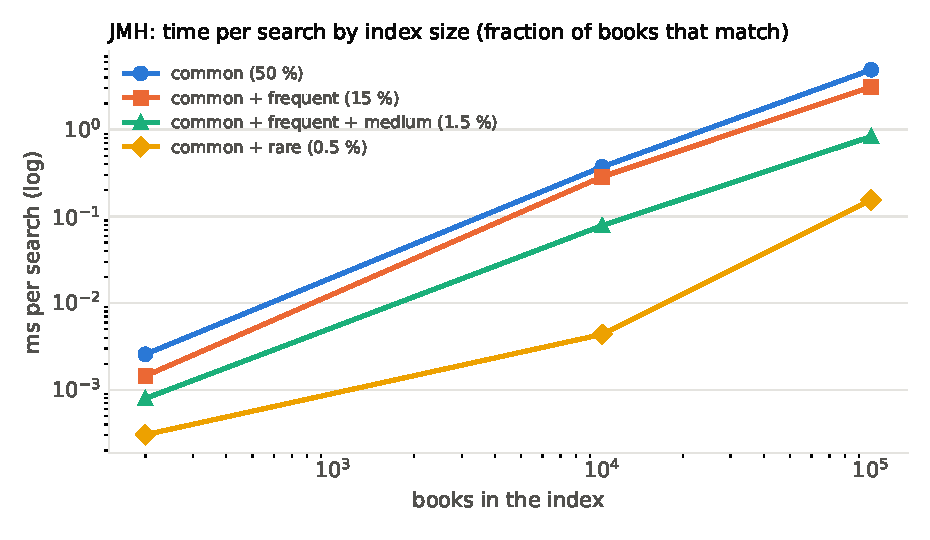
\includegraphics[width=0.82\linewidth]{figures/jmh_intersection.pdf}
\caption{Time per search against the size of the index, both axes logarithmic.}
\end{figure}

\textbf{What the intersection shows.}
\begin{itemize}
  \item \textbf{The cost follows the number of matches, not only the length of the lists.} With 100,000 books the
        four queries all read the list of \code{common}, 50,000 ids, yet they range from 6.06~ms to 0.15~ms. A rarer
        term makes the shortest list shorter, so the intersection walks fewer ids, and fewer matches are then checked
        against the snapshot, filtered and sorted.
  \item \textbf{Ten times more books cost more than ten times as much at the top of the scale.} From 10,000 to
        100,000 books, \code{common} goes from 362~µs to 6.06~ms, 16.7 times. Sorting every match grows faster than
        linearly, and the larger lists no longer fit in the CPU caches. These are our explanations; they were not
        measured separately.
\end{itemize}

\textbf{Filters.} With 100,000 books and the query \code{common}, no filter takes 4.97~ms. The language filter adds
5~\% and the author filter 12~\%, because it compares strings ignoring case; all of them together, 14~\%. The year
filter takes 8~\% less, because it leaves fewer books to sort. Filters run in memory on the metadata of the snapshot,
after the intersection, so they never add a query to MongoDB.

\textbf{Pagination.} The position of the page does not change the cost: with 100,000 books, the first page, the middle
one and one near the end all take about 4.84--4.87~ms, within the error, and so do pages of 100 results. Every search
does all the work (intersection, filters, ordering of every match) before cutting the page, and the cut itself costs
almost nothing. The other side is that the first page is not cheaper either: a user who only looks at 20 results
pays for all of them. Caching the result of a query until the next version is published would avoid it, because a
snapshot never changes.

\begin{figure}[H]
\centering
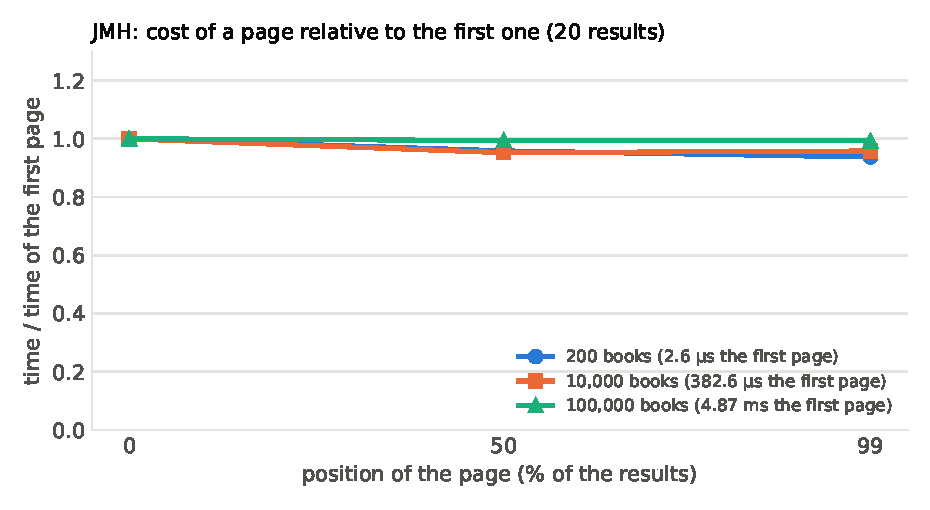
\includegraphics[width=0.82\linewidth]{figures/jmh_pagination.pdf}
\caption{Time of a page relative to the first page, pages of 20 results.}
\end{figure}

\textbf{Threads.} \code{SearchEngine} has no state of its own and the snapshot is immutable, so several threads
search at once without locks. With 100,000 books and \code{common frequent}, 2 threads complete 1.9 times as many
searches per second as one, 4 threads 3.6 times and 8 threads 5.7 times. Each search becomes slower as threads are
added, from 3.31~ms with one to 4.62~ms with eight. The threads do not wait for each other, but they share the CPU
caches and the memory bandwidth, and 8 threads exceed the 6 physical cores of the machine.

\begin{figure}[H]
\centering
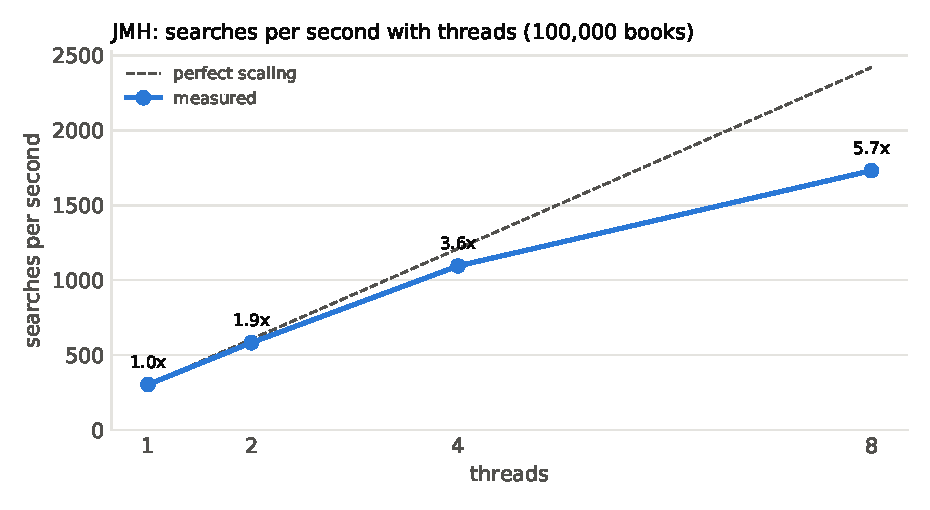
\includegraphics[width=0.82\linewidth]{figures/jmh_threads.pdf}
\caption{Searches per second with 1 to 8 threads, against perfect scaling.}
\end{figure}

This is the cost of the code alone. A real search adds MongoDB, which returns the posting lists, HTTP and nginx: the
load tests measure them.

\subsection{Load tests}

\code{LoadGenerator} sends \code{GET /search} through nginx with \code{shared/queries.txt}, and checks each answer
against the total and version it obtained first: more replicas must not change the results. Before measuring, the
script runs \code{validate-api.sh}. Each configuration is repeated 3 times with 15~s of warm-up and 30~s of measure,
and one factor changes at a time:

\begin{table}[H]
\centering\small
\begin{tabularx}{\linewidth}{@{}L{1.9cm}L{5.2cm}X@{}}
\toprule
\textbf{Experiment} & \textbf{What changes} & \textbf{Fixed} \\
\midrule
Clients & 1, 8, 32, 128, 256 clients with 1, 2 and 4 replicas & 250 threads, pool of 50, nginx with 2 CPUs \\
Threads & 16 and 64 Jetty threads, with the same clients & 1 replica, pool of 50, nginx with 2 CPUs \\
Pool & 10 and 100 MongoDB connections, with 32, 128 and 256 clients & 1 replica, 250 threads, nginx with 2 CPUs \\
nginx & 0.5 CPUs, the limit of the deployment, with 32, 128 and 256 clients & 1 replica, 250 threads, pool of 50 \\
Index size & 200 real books, and 100,000 synthetic ones if available & Same as the clients experiment \\
\bottomrule
\end{tabularx}
\caption{Load experiments. Client concurrency, threads per process and replicas are kept apart.}
\end{table}

\textbf{Why nginx has 2 CPUs here.} Short trial runs showed that nginx, with the 0.5 CPUs of the deployment,
saturated before Search and hid the effect of everything else. The experiments therefore give it 2 CPUs and measure
the 0.5 limit separately.

\textbf{Limitations.}
\begin{itemize}
  \item The generator runs on the same machine as the system, so it competes with it for CPU.
  \item It is a closed loop: under saturation, clients wait instead of queuing more requests, so latencies are lower
        than with requests arriving at a fixed rate.
  \item With 4 replicas the limits of the containers add up to 14 CPUs, which may exceed the host. Then the limits no
        longer bound each container, and the replicas compete for the same cores.
\end{itemize}

\pending{Insert the tables and figures of \code{results/analysis/}: throughput and p95 against clients for each number
of replicas, the effect of threads and of the pool, and CPU and memory per container.}

\subsection{Analysis}

\pending{Write it from the measures, without assuming the outcome. It must answer: at how many clients does the
throughput stop growing, and what happens to p95 and p99? Which container reaches its CPU limit first (Search, MongoDB
or nginx)? Do replicas and threads help, and if not, why? Is the pool of 50 connections too small or too large, as this
was an estimate? Does a larger index move the bottleneck to MongoDB? Were there errors or wrong results?}

\pending{State what was not measured and why: full pipeline under load, 100,000 books if DR-16 did not arrive.}
